\documentclass{school-22.211-notes}
\date{May  7, 2012}

\begin{document}
\maketitle

\lecture{Homogenization Methods}
We continue our discussion on nodal methods, and focus on homogenization methods. This lecture follows closely on Smith's `Assembly Homogenization Techniques for Light Water Reactor Analysis' (Prog. in Nulear Energy, 1986). 

\topic{Nodal Methods: Burnup Dependence}
\begin{enumerate}
\item Spatial configuration matters because of the following three terms vary with respect to space:
\begin{itemize}
\item Burnup gradients: quadratic variation of cross sections with respect to exposure; we integrate bundle surface burnups;
\item Fuel temperature gradients: fuel temperature is related to the local fission rate; and Doppler feedback is from fuel temperature variations;
\item Non-uniform density gradients: coolant feedback is caused by density distribution.
\end{itemize}
For instance, if we know the fuel temperature gradient, from any library we know the cross section change with respect to temperature, then we can compue the cross section distribution.  There are spectral interaction between assemblies. It is very easy to integrate in NEM nodal method, but not so easy with ANM and SANM because of the polynomials. 

\item Space-dependent XS Changes Flux. Recall that for 1 nodal balance equation and 2 incoming current BCs, and the two additional conditions come from the weighted residual method. Now that we add in the spatial dependency of the cross sections, the weighted residual method for 1D neutron diffusion equation remains the same: 
\eqn{ \int_0^1 w(\xi) \left( - \Sigma_D \ddxin2 \psi(\xi) + \Sigma_r (\xi) \psi(\xi) \right) \dxi   \int_0^1 \left( \frac{1}{\keff} \chi(\xi) \psi(\xi) + S(\xi) - L(\xi) \right) \dxi  }
Again, we set the 1st moment of neutron diffusion equation to zero, hence deriving an expression for $a_3$, 
\eqn{ \int_0^1 P_1(\xi) \left( - \Sigma_D \ddxin2 \psi(\xi) + \Sigma_r (\xi) \psi(\xi) - Q(\xi) \right) \dxi &= 0, &a_3&=\frac{5 q_1 + 3 q_3 - 5a_1 \Sigma_r + \cdots}{3(60 \Sigma_D + \Sigma_r) + \cdots} }
Similarly we set the 2nd moment of neutron diffusion equaion to zero, hence deriving an expression for $a_4$, 
\eqn{ \int_0^1 P_2(\xi) \left( - \Sigma_D \ddxin2 \psi(\xi) + \Sigma_r (\xi) \psi(\xi) - Q(\xi) \right) \dxi &= 0, &a_4&=\frac{-7q_2 + 3 q_4 + 7 a_2 \Sigma_r + \cdots}{420(\Sigma_D + 3\Sigma_r) + \cdots} }
Interpretations: flux distribution changes after we add in the spatial dependency of cross sections; but mechanically there is nothing tricky: we are just adding more terms, designated by $\cdots$, to the expressions in the above two equations. 

\item Depletion benchmark using BOC-2 Powers: without space-dependent xs, the error on $\keff$ is about 12pcm (on the edge); with space-dependent xs, the error on $\keff$ drops to about 4pcm (on the edge). The error on the interior is always smaller. 
\end{enumerate}

\clearpage
\topic{Homogenization of Fuel Assemblies}
Homogenization theory: 
\begin{enumerate}
\item Given a reference solution, we build a heterogeneous reactor using,
\eqn{ \divergence \vecJ_g(\vecr) + \Sigma_{tg}(\vecr) \phi_g(\vecr) &= \Sum_{g'=1}^G \left( \frac{1}{\keff} M_{gg'} (\vecr) + \Sigma_{gg'} (\vecr) \right) \phi_{g'} (\vecr) }
and analogous equation for the homogenized model using homogenized parameters,
\eqn{ \divergence \hat{\vecJ}_g(\vecr) + \hat{\Sigma}_{tg}(\vecr)\hat{\phi}_g(\vecr) &= \Sum_{g'=1}^G \left( \frac{1}{\keff} \hat{M}_{gg'} (\vecr) + \hat{\Sigma}_{gg'} (\vecr) \right) \hat{\phi}_{g'} (\vecr) }

\item We cannot preserve every term, but we can decide to preserve some. For instance, we preserve the scalar flux, reaction rates ($\alpha = t, gg'$ etc) and the leakage term, 
\begin{align}
\int \hat{\phi}_g \dr &= \int \phi_{Ag} \dr  \\
\int_{V_i} \hat{\Sigma}_{\alpha g} \hat{\phi}_g \dr &= \int_{V_i} \Sigma_{\alpha g} \phi_g \dr  & \hat{\Sigma}_{\alpha g}^i &= \frac{\int_{V_i} \Sigma_{\alpha g} \phi_g \dr}{\int_{V_i} \hat{\phi}_g \dr} \\
\int_{S_i^k} \divergence \hat{J}_g \dS &= \int_{S_i^k} \divergence \vecJ_g \dS & \hat{J}_g &= - \hat{D}_g \gradient \hat{\phi}_g, \mbox{ where } \hat{D}_g^i = \frac{-\int_{S_i^k} \vecJ_g \dS}{\int_{S_i^k} \gradient \hat{\phi}_g \dS}
\end{align}

\item AXS (flux-weighted cross sections) vs. RXS (reference cross sections): Homogenization by itself introduces errors: -0.44\% for $\keff$, 5.5\% for average assembly power. These errors do not really decrease as we decrease the mesh size; they do not go away neither if we use perfect cross sections (RXS): -0.34\% for $\keff$, 4.1\% for average assembly power. As we will examine in the next section, the errors have to do with the discontinuity of scalar flux. 

\item Flux discontinuity: since the homogenized flux distribution in each node is affected by the diffusion coefficients, and the choice of flux weighted diffusion coefficients is in a sense entirely arbitrary, the interface fluxes can be different as in Figure~\ref{1Dnodal-flux}(c). As a direct result, the homogenized flux in nodes $i, i+1$ when the two-node homogenized diffusion problem is solved with BCs $J_i^-, J_{i+1}^+$ and continuity of flux and current interface conditions would yield Figure~\ref{1Dnodal-flux}(d), which is different from Figure~\ref{1Dnodal-flux}(c). That is, the homogeneous flux is not continuous across the surface anymore. 
\begin{figure}[ht]
  \centering
  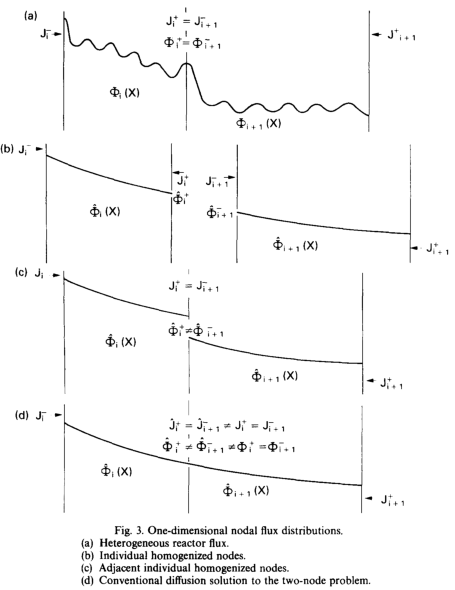
\includegraphics[width=4in]{images/methd/1Dnodal-flux.png}
  \caption{Nodal Flux Distribution} \label{1Dnodal-flux}
\end{figure}

\item Heterogeneity factor(HF): Koebke introduced the \hi{Heterogeneity Factor}(Lugano, 1978), which states,
\eqn{ \hat{\phi}_i f_i^+ &= \hat{\phi}_{i+1}^- f_{i+1}^-  \label{nodal-hh}}
where the equivalence factors are defined as (and computed from reference solution), 
\eqn{ f_i^+ &= \frac{\phi_i^+}{\hat{\phi}_i^+}, &f_{i+1}^-&= \frac{\phi_{i+1}^-}{\hat{\phi}_{i+1}^-}}
which says that the heterogeneous flux is continuous across the interface and that there exists a direct relationship between the heterogeneous and homogenized surface fluxes. When the homogenized two-node problem is solved, the homogenized flux is made discontinuous (by a factor of $f_i^+/f_{i+1}^-$) and the homogenized flux distribution will be the same as that in Fig.~\ref{1Dnodal-fulx}(c), which results in the \textit{preservation of interface current}. 

\item Nodal equivalence theory and discontinuity factor(DF): Koebke's method of constraining the diffusion coefficients such that the heterogeneity factors are identical on both surfaces of a node requires an iterative method to determine diffusion coefficients. A variation of Koebke's method takes advantage of the fact that exact heterogeneity factors can be defined from Eq.~\ref{nodal-hh} for any value of the diffusion coefficient. Note that unless the diffusion coefficients are found iteratively, the values of the heterogeneity factors on the opposite faces of a node will be different. These two factors are referred to as \hi{discontinuity factor}(DF) to distinguish them from heterogeneity factors, 
  \eqn{ f_{gi,j}^{u-} &= \frac{\phi_{gi,j}^u (u_l)}{\hat{\phi}_{gi,j}^u (u_l)}, &f_{gi,j}^{u+} &= \frac{\phi_{gi,j}^u (u_{l+1})}{\hat{\phi}_{gi,j}^u (u_{l+1})} }
  where $u_l, u_{l+1}$ are the lower and upper $u$-direction boundaries of node $i,j$. 

\item Application of DF: Koebke modified the NEM code, demonstrating that heterogeneous reference solutions could be reproduced by using heterogeneity factors; Smith modifed the QUANDRY code, demonstrating that even CMFD method could reproduce heterogeneous reference solution using discontinuity factors. The updated nodal interface current on the upper $u$-direction surface of node $i,j$ in the CMFD approximation is,
  \eqn{ \hat{J}_{gi,j}^u = \frac{2D_{i,j} D_{i+1,j}}{h_i h_{i+1}} \frac{f_{gi,j}^{u+} \hat{\phi}_{gi,j} - f_{gi+1,j}^{u-} \hat{\phi}_{gi+1,j}}{h (f_{gi+1,j}^{u-} + f_{gi,j}^{u+})} }
  which is different from the traditional CMFD current, 
  \eqn{ \hat{J}_{gi,j}^u = \frac{2D}{h} \left[ \hat{\phi}_{gi,j} - \hat{\phi}_{gi+1,j} \right] }
  Notice the heterogeneity-modified-CMFD is different from the traditional CMFD in the sense that the coefficients in front of the two flux are not the same anymore. 

\item Assembly Discontinuity Factor (ADF). There exists a homogeneous analogy to the heterogeneous assembly calculation: a single-node problem with zero net current boundary conditions. In the analogous problem, the homogenized fluxes are spatially flat. Since the assembly-averaged fluxes in the homogeneous and heterogeneous assembly calculations are by definition euqal, \textbf{the DFs are simply ratios of the surface-averaged fluxes to the cell-averaged fluxes in the heterogeneous assembly calculation.} 
  \begin{itemize}
  \item It is thus possible to approximate all of the equivalence parameters, assembly discontinuity factors (ADFs), by perfoming assembly calculations for each type of assembly. 
  \item For the HAFAS problem, the ADFs are within a few percent of the mean values of the reference discontinuity factor (RDFs) for all assembly types. Moreover, the fast group DFs are much closer to unity than are the thermal group DFs; the wide gap DFs are much different than the narrow gap DFs. 
  \item The good agreement between ADFs and RDFs suggests that DFs are insensitive to the assembly position, and ADFs can be computed directly from the information available in standard assembly calculations. 
  \item ADFs dramaticaly reduce errors in both PWRs and BWRs. 
  \item The AXS-ADF combination is important in that it is more accurate than either RXS-ADF or AXS-RDF. Part of the reason AXS-ADF is more accurate is that ADF and AXS tend to have erros opposite in signs. Keep in mind that reference xs (RXS) is not sufficient to reduce errors. 
  \end{itemize}
\end{enumerate}

\clearpage
\topic{Application of DFs: Reflector Modeling}
PWR baffle/reflector (about 1.5in thick stainless steel outside the core) is non-trival to model because historically nodal models have used empirical albedos to replace the baffle and reflector. Determination of albedos involves a length trial and error procedure until the nodal power matches that of some higher-order solution. After improvements in nodal models, the difficulty became finding appropriate homogenized parameters for baffle/reflector nodes. Since the baffle is a strong absorber, using flux-volume weighted cross sections distributes the absorption over the entire baffle/reflector region, which can lead to error in power distribution as large as 10-15\%. 

We turn to DFs because they are less spatially sensitive than albedos (as shown in Table 12 in Smith's paper, DF is more or less the same at different nodes). A typically treatment involves, 
\begin{itemize}
\item Use an assembly homogenization code (for instance CASMO) to model one or more fuel assemblies, the baffle, and reflector; 
\item Collapse baffle cross sections into two groups to assure that finite difference diffusion calculation would reproduce the transport results;  
\item Use flux, current distribution and reaction rates directly to define homogenized cross sections and DFs, which accurately model the baffle and reflector. 
\end{itemize}
The inherent advantage of HFs or DFs is that they are chosen in such a way that the nodal model would reproduce the net currents at the core/baffle interface and the net reaction rates in both the fuel assembly and the homogenized baffle/reflector without explicitly representing the baffle. It turns out that for reflector purpose, the fast neutron leakage makes up for 90\% of the leakage, and it is very insensitive to enrichment, burnup etc. 

Application and Limitation of DFs:
\begin{itemize}
\item Other geometries: Assembly/Reflector DFs also work in hexagonal geometry. 
\item Other reactor types: DFs may not work because graphite or gas or fast reactor the mean free path is long. DFs work well mostly for thermal LWRs. 
\end{itemize}

Other applications of homogenization theory: 
\begin{itemize}
\item Fine mesh data generation for 3D/1D axial models. Basically we homogenize axial fuel asembly, and depens on how we define the node, the DFs come out to be different. 
\item Nonlinear acceleration of fine-mesh transport methods. 
\item Nonlinear acceleration of Monte Carlo. 
\end{itemize}

\clearpage
\topic{Summary of Homogenization Theories}
Homogenization theories:
\begin{enumerate}
\item We would love to solve for the reference fluxes with all the detailed up and downs; but we can only solve down to the level of nodal fluxes; to estimate the discontinuity conditions of nodal fluxes in two neihboring nodes, we use HF/DFs. We don't care that the nodal fluxes are discontinuous; all we care is the re-constructed fluxes. 
\item Homogenization is required any time spatial reduction is employed, be it at the pin-cell level, assembly level, assembly clusters (BWRs); 
\item Exact homogenization parameters depend on reference solutions, which are seldome available and certainly self-defeating;
\item Exact homogenization parameters depend slightly on details of the nodal spatial model;
\item Homogenization for transport methods is not as simple as for diffusion methods;
\item Methods more accurate than simple AXS/ADFs are very desirable to further improve accuracy. 
\end{enumerate}

\end{document}
